\documentclass[brazil, a4paper,12pt]{article}
\bibliographystyle{plain}
\usepackage[brazil]{babel}
\usepackage{graphicx}
\usepackage{geometry}
\usepackage[utf8]{inputenc}
\usepackage[T1]{fontenc}
\usepackage{listings}
\usepackage{indentfirst}
\usepackage{lmodern}
\geometry{a4paper,left=3cm,right=3cm,top=2.5cm,bottom=2.93cm}

\lstset{numbers=left,
stepnumber=0,
firstnumber=1,
numberstyle=\tiny,
extendedchars=true,
breaklines=true,
frame=tb,
tabsize=2,
basicstyle=\footnotesize,
stringstyle=\ttfamily,
showstringspaces=false
}

\renewcommand{\lstlistingname}{Programa}

\begin{document}
\begin{titlepage}

  \vfill

  \begin{center}
    \begin{large}
      Universidade Federal de Ouro Preto
    \end{large}
  \end{center}

  \begin{center}
    \begin{large}
      Instituto de Ciências Exatas e Aplicadas
    \end{large}
  \end{center}

  \begin{center}
    \begin{large}
      Departamento de Computação e Sistemas
    \end{large}
  \end{center}

  \vfill

  \begin{center}
    \begin{Large}
      \textbf{REDES DE COMPUTADORES 1\\[0.4cm] 
        Primeiro Trabalho}               
    \end{Large}
  \end{center}


  \vfill

  \begin{center}
    \begin{large}
    	
   	  Guilherme Marx Ferreira Tavares - 14.1.8006
   	  
   	  Rafael Júnio Cota Cekiera - 14.2.5834

       \end{large}
  \end{center}

  \begin{center}
    \begin{large}
      Professor - Theo Lins
    \end{large}
  \end{center}

  \vfill

  \begin{center}
    \begin{large}
      João Monlevade \\
      \today \\
    \end{large}
  \end{center}

\clearpage
\tableofcontents 
\end{titlepage}

%--------------------------------------------------------


\section{Introdução}
Neste trabalho prático, que tem a finalidade de aplicar o conceito de socket em redes de computadores, deve-se implementar uma comunicação entre processos situados em sistemas diferentes por meio do mecanismo socket.


\section{Algoritmos}
Um processo Cliente deve transmitir dois números e uma operação para o processo Servidor que, por sua vez, deve realizar a operação desejada entre os dois números e retornar ao cliente o resultado correto.

\subsection{Servidor}
\begin{itemize}
 	\item Primeiramente o servidor é iniciado na porta $55555$, agora ele entra em estado de espera aguardando pela chamada da conexão do cliente.
	\item Uma vez recebida a solicitação de conexão, o servidor a aceita.
	\item O servidor recebe a mensagem do cliente contendo os dois valores e a operação por meio de uma string codificada em UTF, via TCP.
	\item O servidor decodifica a mensagem do cliente, colocando os valores em duas variáveis inteiras e fazendo seu calculo de acordo com o char contido no local da operação.
	\item Uma vez o resultado caculado, o servidor o coloca em uma nova String e a envia para o cliente novamente com codificação UTF com uso do protocolo TCP.
	\item O servidor encerra a conexão com o cliente e se fecha.
\end{itemize}

\subsection{Cliente}
\begin{itemize}
	\item O cliente solicita os valores e a operação a ser realizada para o usuário e as salva em uma string.
	\item O cliente se conecta ao servidor na porta $55555$ e envia ao servidor a string contendo os valores e a operação em formato UTF utilizando protocolo TCP.
	\item Cliente entra em modo de espera, aguardando a resposta do servidor. 
	\item Ao obter a resposta do servidor, o cliente exibe essa resposta ao usuário, fecha sua conexão e finaliza.
	
\end{itemize}

\newpage
\section{Apresentação e discussão dos resultados}
Foram realizado os testes de funcionamento do programa:

\begin{itemize}
	\item Teste programa: 
	
	\begin{figure}[ht!]
		\centering
		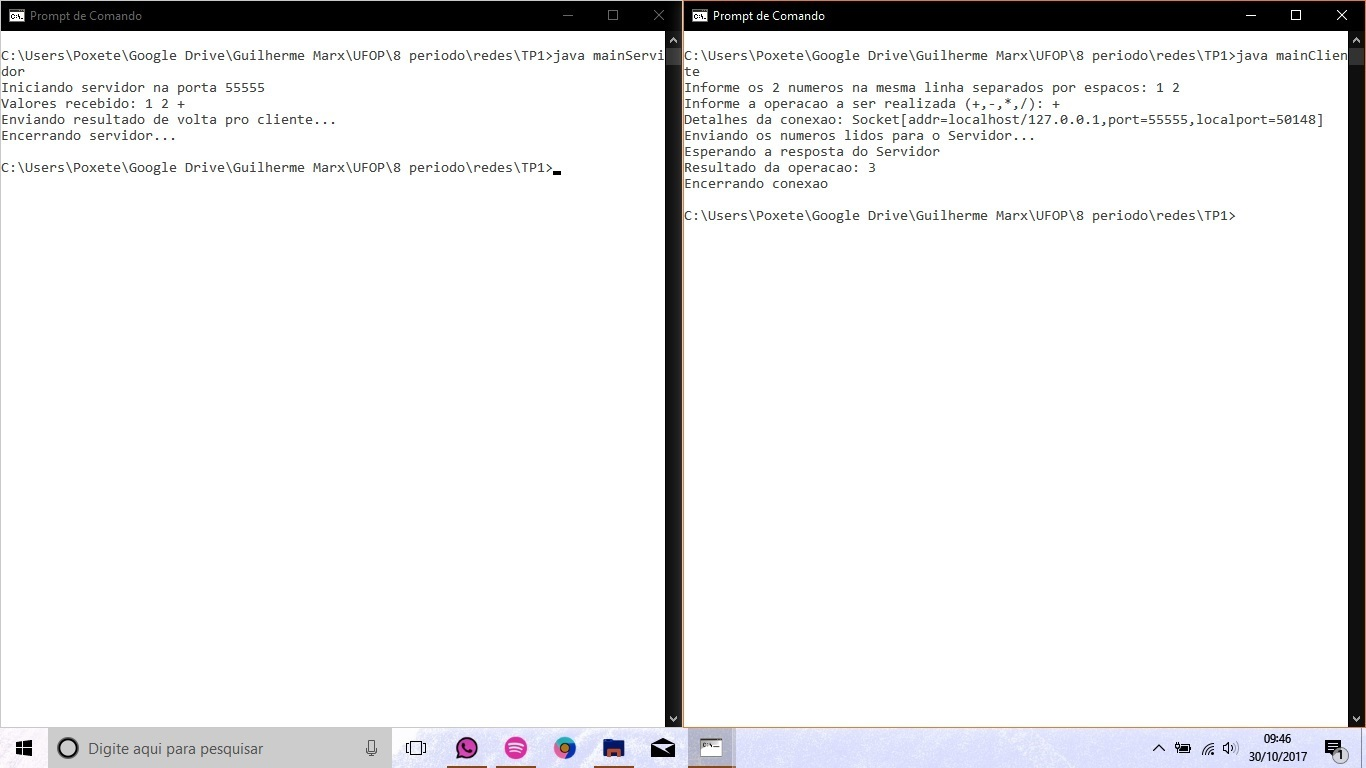
\includegraphics[scale=0.45]{teste1.jpg}
		\caption{Tela do teste}
		\label{Rotulo}
	\end{figure}
	
	Foi constatado que somando dois valores positivos, o programa não obteve problemas.
	
	\newpage

	\begin{figure}[ht!]
		\centering
		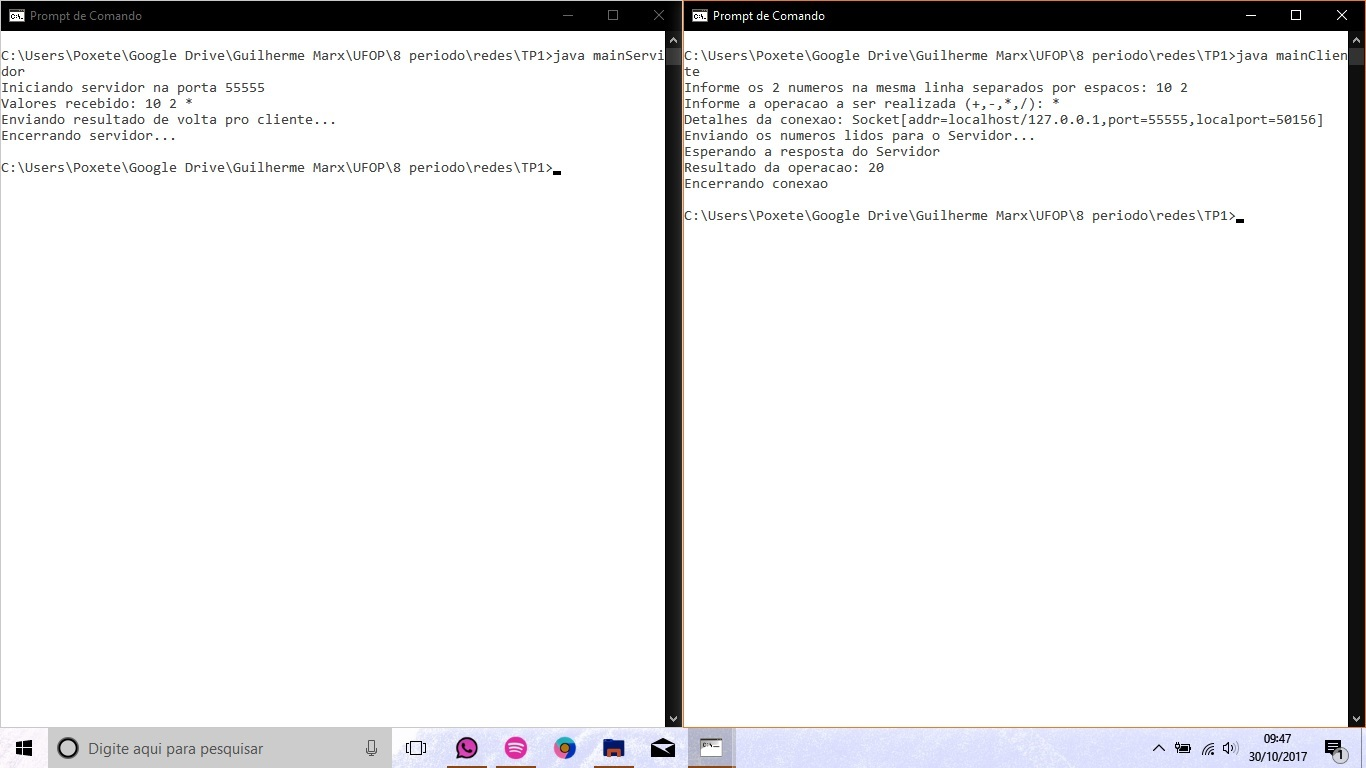
\includegraphics[scale=0.45]{teste2.jpg}
		\caption{Tela do teste}
		\label{Rotulo}
	\end{figure}
	
	Foi constatado que multiplicando dois valores positivos, o programa não obteve problemas.
	
	\newpage	
	
	\begin{figure}[ht!]
		\centering
		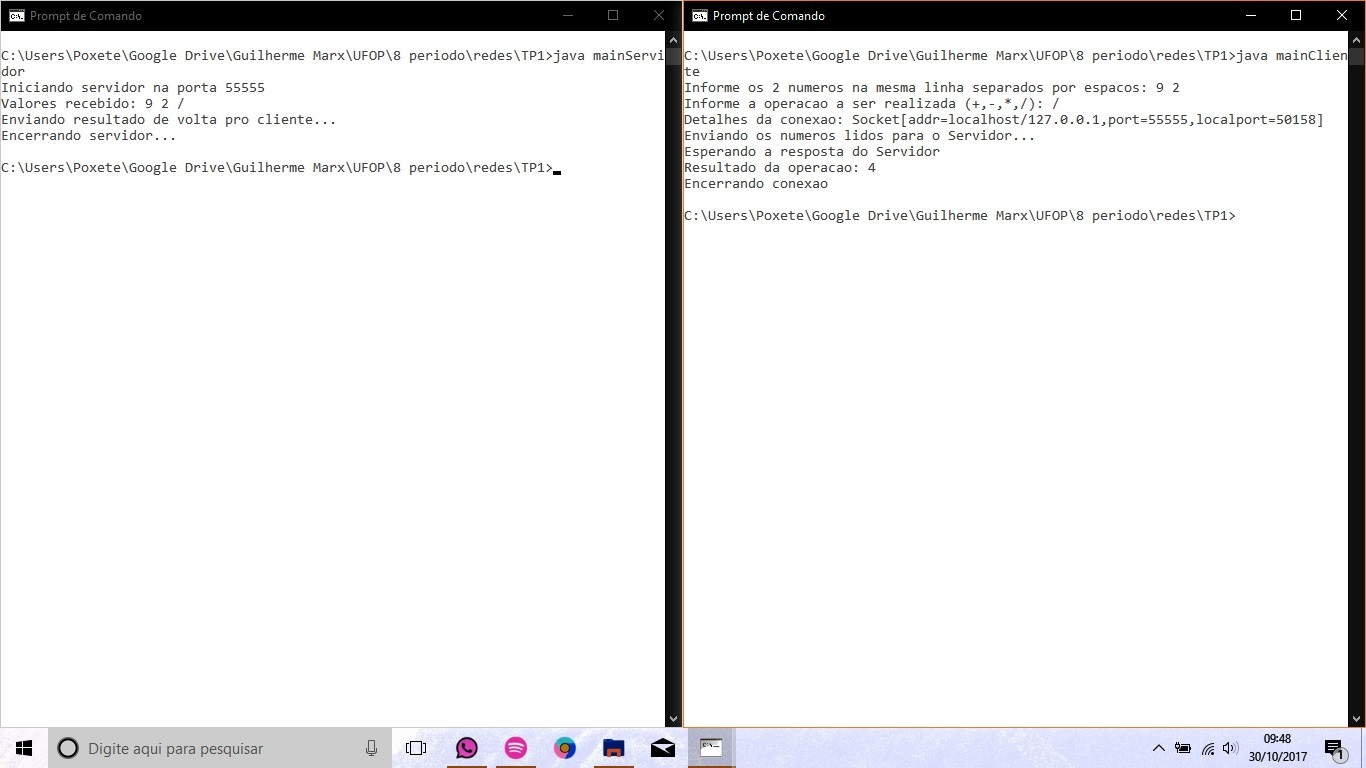
\includegraphics[scale=0.45]{teste3.jpg}
		\caption{Tela do teste}
		\label{Rotulo}
	\end{figure}
	
	Foi constatado que no momento da divisão, o programa desconsidera as casas decimais do resultado. Isso é pelo fato de que as variáveis dentro do programa eram inteiras, então no momento da divisão é feita uma divisão inteira e não uma divisão com parte fracionária.
	
	\newpage
	
	\begin{figure}[ht!]
		\centering
		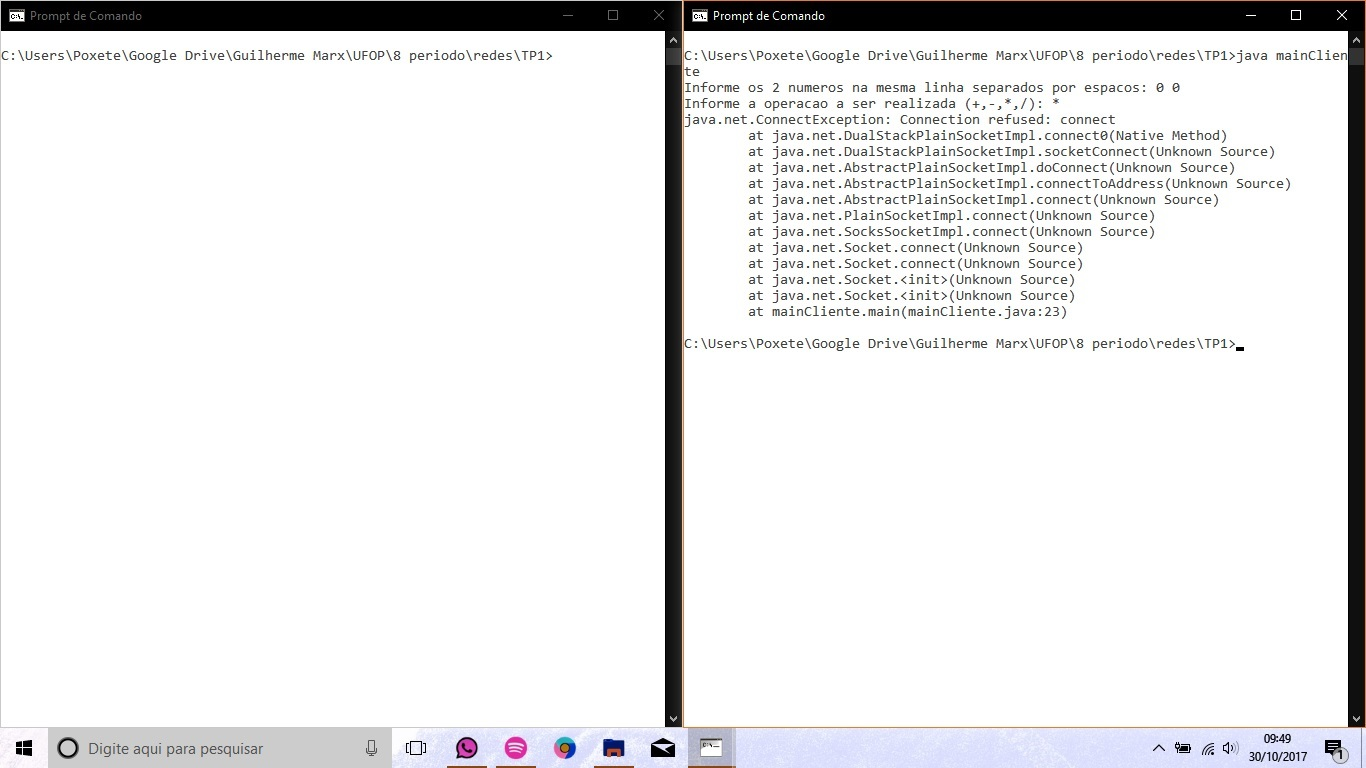
\includegraphics[scale=0.45]{teste4.jpg}
		\caption{Tela do teste}
		\label{Rotulo}
	\end{figure}
	
	Foi constatado que temos um crash no processo do cliente quando ele tenta conectar o servidor que não foi iniciado.
	
	\newpage
	
	\begin{figure}[ht!]
		\centering
		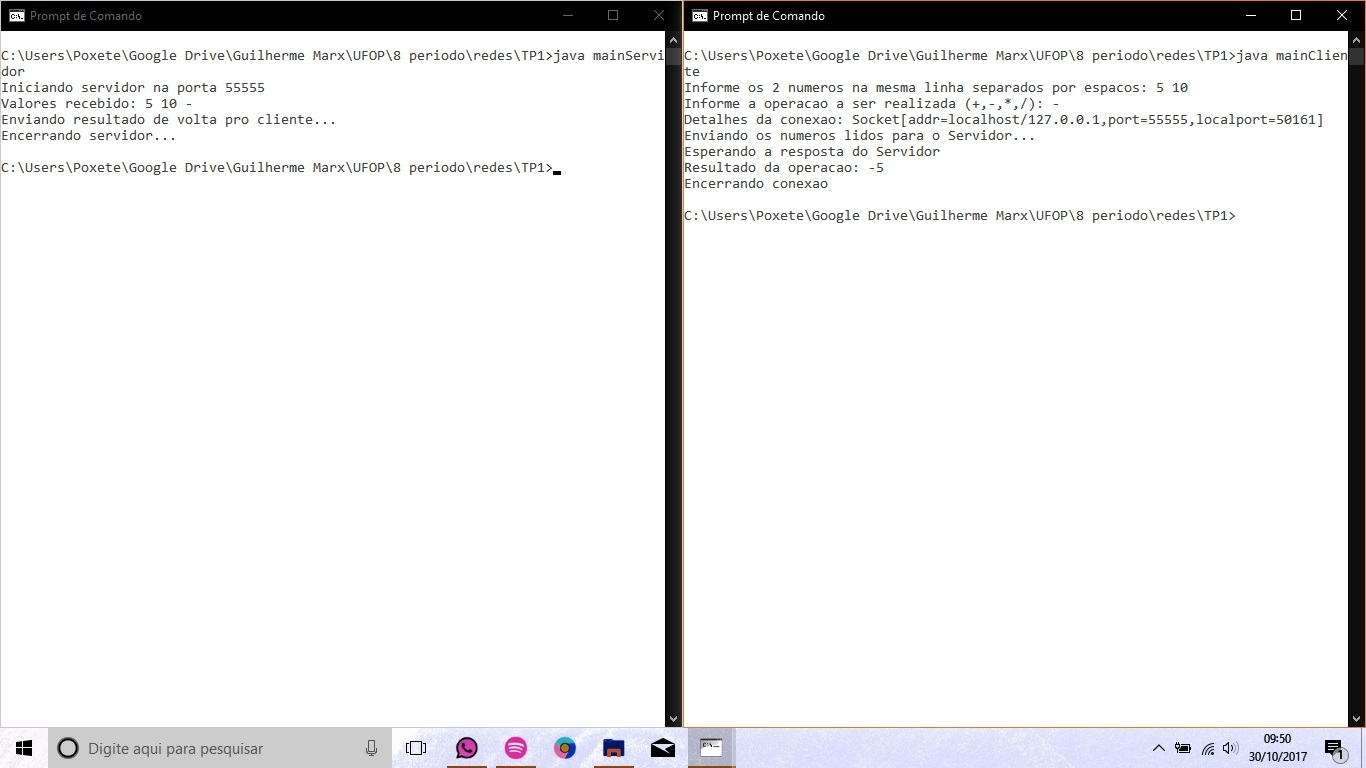
\includegraphics[scale=0.45]{teste5.jpg}
		\caption{Tela do teste}
		\label{Rotulo}
	\end{figure}
	
	Foi constatado que quando o resultado deve ser negativo, o programa não obteve nenhum problema.
	
	\newpage
	
	\begin{figure}[ht!]
		\centering
		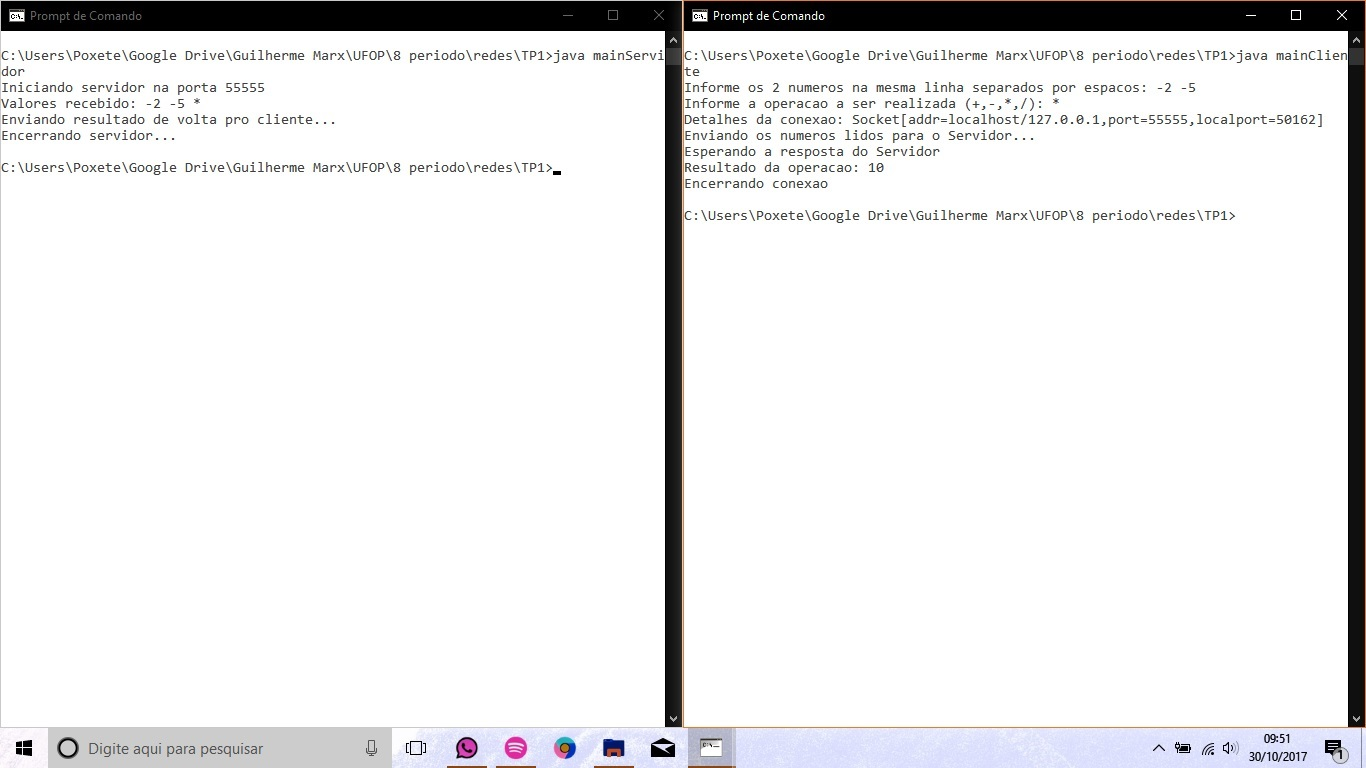
\includegraphics[scale=0.45]{teste6.jpg}
		\caption{Tela do teste}
		\label{Rotulo}
	\end{figure}
	
	Foi constatado que quando se usa valores negativos no programa, ele não obteve nenhum problema.
	
	\newpage

	\begin{figure}[ht!]
		\centering
		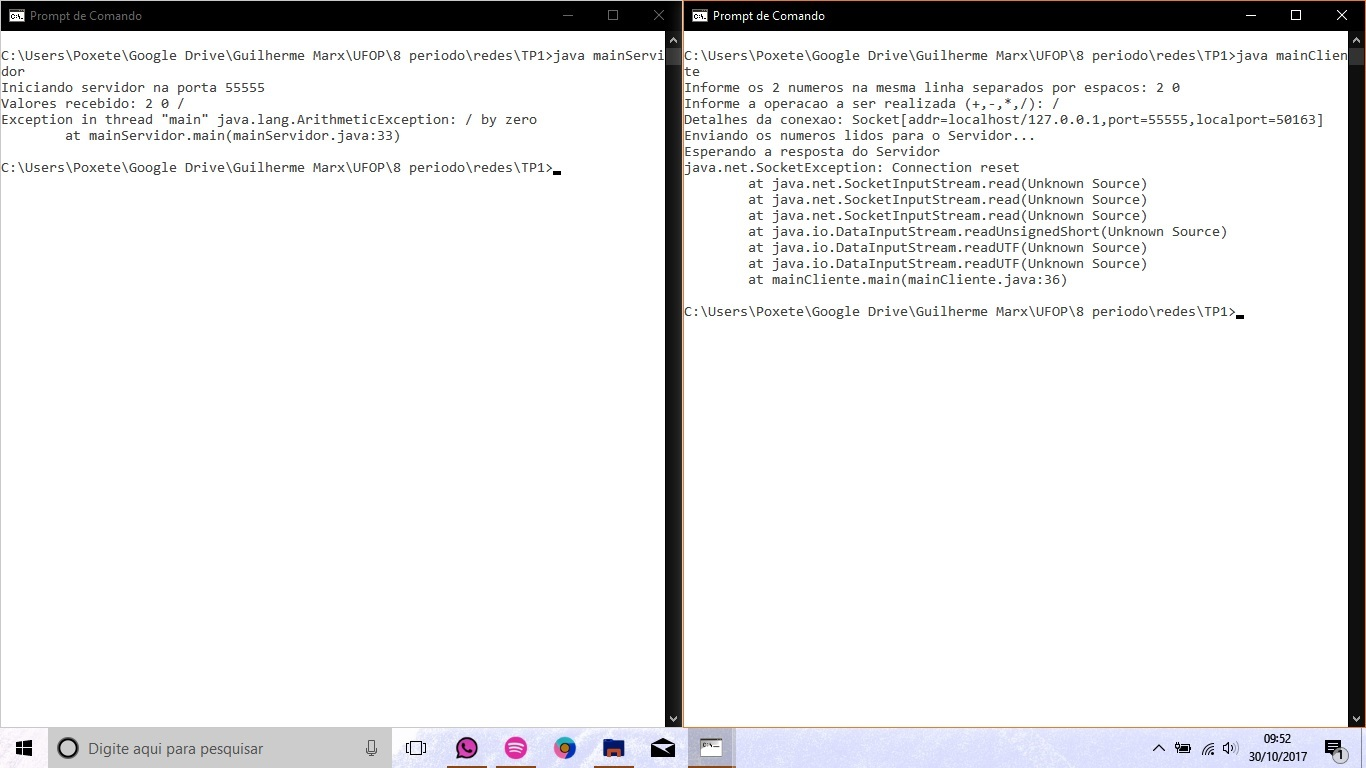
\includegraphics[scale=0.45]{teste7.jpg}
		\caption{Tela do teste}
		\label{Rotulo}
	\end{figure}
	
	Foi constatado que o processo servidor dava crash quando a operação a ser realizada era uma divisão por zero. Por esse motivo, no momento da operação de divisão foi incluído um novo fluxo de execução, pois assim, consegue-se separar a divisão por zero de uma divisão normal.
	
	\newpage
	
	\begin{figure}[ht!]
		\centering
		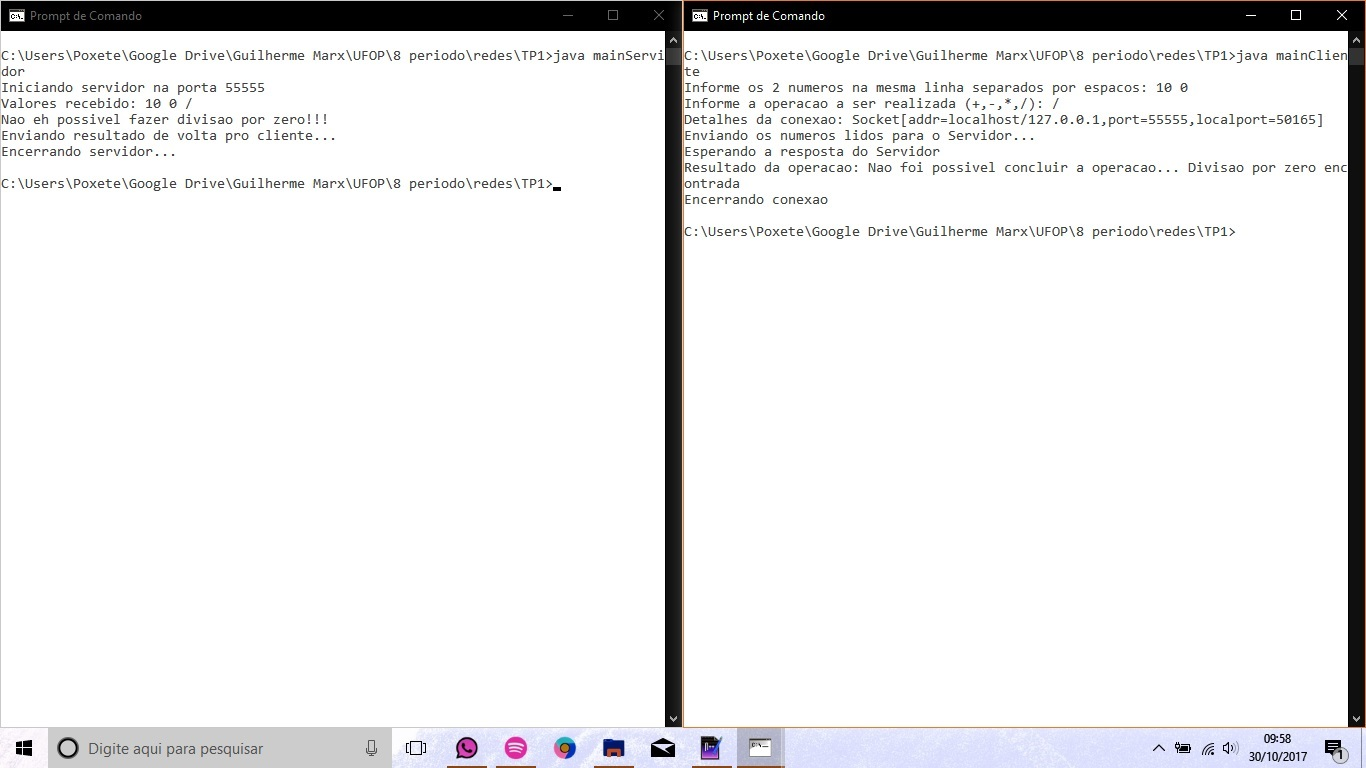
\includegraphics[scale=0.45]{teste8.jpg}
		\caption{Tela do teste}
		\label{Rotulo}
	\end{figure}
	
	Novo teste da divisão por zero, agora após o novo fluxo ser adicionado no servidor. No teste podemos ver que nenhum dos processos dá crash nessa situação, o problema foi resolvido.
	
	\newpage
	
\end{itemize}

\newpage		
\subsection{Discussão dos resultados}
Vemos com esses testes que o único problema que esse programa pode ter é quando o cliente é iniciado antes do servidor, ou seja, quando o cliente solicita a conexão ao servidor com este ainda fechado. 

A divisão por zero foi relativamente simples de se resolver, colocou-se um condicional para garantir que a divisão só seja feita quando o valor do denominador não for zero e uma bandeira para avisar quando isso acontecer ou não para, caso realmente tenha-se tido uma divisão por zero, não deixar o cliente sem uma resposta.

\section{Apêndice A}
\lstinputlisting[language=java, label=cod:mainServidor.java, caption={mainServidor.java}]{mainServidor.java}
\lstinputlisting[language=java, label=cod:mainCliente.java, caption={mainCliente.java}]{mainCliente.java}

\newpage
\section {Bibliografia}

\noindent[1] TENENBAUM, AARON M. Estruturas de dados usando C / AARON M. TENEMBAUM,
YEDIDYAH LANHSAM, MOSHE J. AUGENSTEIN; São Paulo : MAKRON Books, 1995.
\newline

\noindent[2] KUROSE, J. F. e ROSS, K.  Redes de Computadores e a Internet / KUROSE, J. F. e ROSS, K;  5ª Ed., Pearson, 2010.
\newline

\noindent[3] HARVEY M. DEITEL \& PAUL J. DEITEL.  Java como programar / HARVEY M. DEITEL \& PAUL J. DEITEL, K;  8ª Ed., Prentice Hall - Br, 2010.

\end{document}
